%\subsection{Exercice 2 (6 points)}\label{exercice-2-6-points}

\emph{Cet exercice porte sur les arbres binaires de recherche, la POO et
la récursivité.}

Nous disposons d'une classe \texttt{ABR} pour les arbres binaires de
recherche dont les clés sont des entiers :

\begin{Shaded}
\begin{Highlighting}[]
\DecValTok{1} \KeywordTok{class}\NormalTok{ ABR():}
\DecValTok{2}   \KeywordTok{def} \FunctionTok{\_\_init\_\_}\NormalTok{(}\VariableTok{self}\NormalTok{) :}
\DecValTok{3}       \CommentTok{\# Initialise une instance d\textquotesingle{}ABR vide.}
\DecValTok{4}
\DecValTok{5}   \KeywordTok{def}\NormalTok{ cle(}\VariableTok{self}\NormalTok{):}
\DecValTok{6}       \CommentTok{\# Renvoie la clé de la racine de l\textquotesingle{}instance d\textquotesingle{}ABR.}
\DecValTok{7}
\DecValTok{8}   \KeywordTok{def}\NormalTok{ sad(}\VariableTok{self}\NormalTok{):}
\DecValTok{9}       \CommentTok{\# Renvoie le sous{-}arbre droit de l\textquotesingle{}instance d\textquotesingle{}ABR.}
\DecValTok{10}
\DecValTok{11}  \KeywordTok{def}\NormalTok{ sag(}\VariableTok{self}\NormalTok{):}
\DecValTok{12}      \CommentTok{\# Renvoie le sous{-}arbre gauche de l\textquotesingle{}instance d\textquotesingle{}ABR.}
\DecValTok{13}
\DecValTok{14}  \KeywordTok{def}\NormalTok{ est\_vide(}\VariableTok{self}\NormalTok{):}
\DecValTok{15}      \CommentTok{\# Renvoie True si l\textquotesingle{}instance d\textquotesingle{}ABR est vide et False sinon.}
\DecValTok{16}
\DecValTok{17}  \KeywordTok{def}\NormalTok{ inserer(}\VariableTok{self}\NormalTok{, cle\_a\_inserer):}
\DecValTok{18}        \CommentTok{\# Insère cle\_a\_inserer à sa place dans l\textquotesingle{}instance d\textquotesingle{}ABR.}
\end{Highlighting}
\end{Shaded}

Considérons ci-dessous trois arbres binaires de recherche :

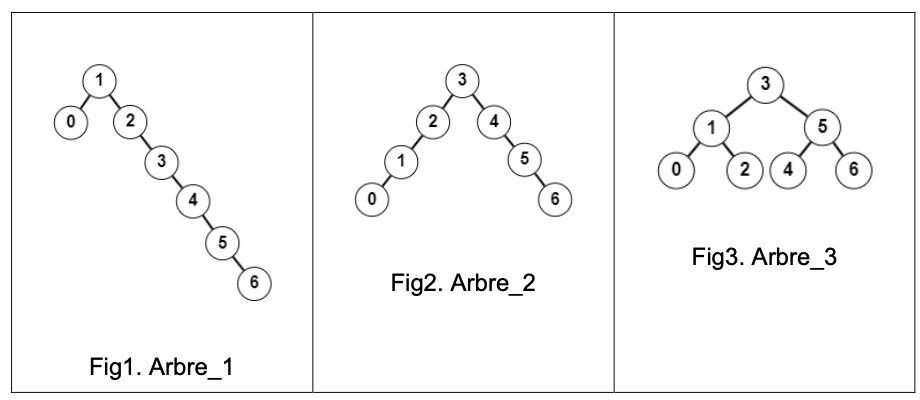
\includegraphics{24-NSIJ2PO1-Ex2-01.png}

Dans tout l'exercice, nous ferons référence à ces trois arbres binaires
de recherche et utiliserons la classe \texttt{ABR} et ses méthodes.

\subsubsection{Partie A}\label{partie-a}

\begin{enumerate}
\def\labelenumi{\arabic{enumi}.}
\tightlist
\item
  Un arbre est une structure de données hiérarchique dont chaque élément
  est un nœud.
\end{enumerate}

\textbf{Recopier} et \textbf{compléter} le texte ci-dessous en
choisissant des expressions parmi \texttt{au\ maximum},
\texttt{au\ minimum}, \texttt{exactement}, \texttt{feuille},
\texttt{racine}, \texttt{sous-arbre\ gauche} et
\texttt{sous-arbre\ droit} :

\begin{itemize}
\tightlist
\item
  Le nœud initial est appelé \ldots{} .
\item
  Un nœud qui n'a pas de fils est appelé \ldots.
\item
  Un arbre binaire est un arbre dans lequel chaque nœud a \ldots{} deux
  fils.
\item
  Un arbre binaire de recherche est un arbre binaire dans lequel tout
  nœud est associé à une clé qui est :

  \begin{itemize}
  \tightlist
  \item
    supérieure à chaque clé de tous les nœuds de son \ldots{}
  \item
    inférieure à chaque clé de tous les nœuds de son \ldots.
  \end{itemize}
\end{itemize}

\begin{enumerate}
\def\labelenumi{\arabic{enumi}.}
\setcounter{enumi}{1}
\item
  Donner dans l'ordre les clés obtenues lors du parcours préfixe de
  l'arbre no 1.
\item
  Donner dans l'ordre, les clés obtenues lors du parcours suffixe,
  également appelé postfixe, de l'arbre no 2.
\item
  Donner dans l'ordre, les clés obtenues lors du parcours infixe de
  l'arbre no 3.
\item
  \textbf{Recopier} et \textbf{compléter} les instructions ci-dessous
  afin de définir puis de construire, en y insérant les clés dans un
  ordre correct (il y a plusieurs possibilités, on en demande une) , les
  trois instances de la classe \texttt{ABR} qui correspondent aux trois
  arbres binaires de recherche représentés plus haut.
\end{enumerate}

\begin{Shaded}
\begin{Highlighting}[]
\DecValTok{1}\NormalTok{ arbre\_no1 }\OperatorTok{=}\NormalTok{ ...}
\DecValTok{2}\NormalTok{ arbre\_no2 }\OperatorTok{=}\NormalTok{ ...}
\DecValTok{3}\NormalTok{ arbre\_no3 }\OperatorTok{=}\NormalTok{ ...}
\DecValTok{4} \ControlFlowTok{for}\NormalTok{ cle\_a\_inserer }\KeywordTok{in}\NormalTok{ [..., ..., ..., ..., ..., ..., ...]:}
\DecValTok{5}\NormalTok{   arbre\_no1....}
\DecValTok{6} \ControlFlowTok{for}\NormalTok{ cle\_a\_inserer }\KeywordTok{in}\NormalTok{ [..., ..., ..., ..., ..., ..., ...]:}
\DecValTok{7}\NormalTok{   arbre\_no2....}
\DecValTok{8} \ControlFlowTok{for}\NormalTok{ cle\_a\_inserer }\KeywordTok{in}\NormalTok{ [..., ..., ..., ..., ..., ..., ...]:}
\DecValTok{9}\NormalTok{   arbre\_no3....}
\end{Highlighting}
\end{Shaded}

\begin{enumerate}
\def\labelenumi{\arabic{enumi}.}
\setcounter{enumi}{5}
\tightlist
\item
  Voici le code de la méthode \texttt{hauteur} de la classe \texttt{ABR}
  qui renvoie la hauteur d'une instance d'ABR:
\end{enumerate}

\begin{Shaded}
\begin{Highlighting}[]
\DecValTok{1} \KeywordTok{def}\NormalTok{ hauteur(}\VariableTok{self}\NormalTok{):}
\DecValTok{2}   \ControlFlowTok{if} \VariableTok{self}\NormalTok{.est\_vide() :}
\DecValTok{3}       \ControlFlowTok{return} \OperatorTok{{-}}\DecValTok{1}
\DecValTok{4}   \ControlFlowTok{else}\NormalTok{ :}
\DecValTok{5}       \ControlFlowTok{return} \DecValTok{1} \OperatorTok{+} \BuiltInTok{max}\NormalTok{(}\VariableTok{self}\NormalTok{.sag().hauteur(),}
\DecValTok{6}                       \VariableTok{self}\NormalTok{.sad().hauteur())}
\end{Highlighting}
\end{Shaded}

Donner, \textbf{en utilisant cette méthode}, la hauteur des trois
instances arbre\_no1, arbre\_no2 et arbre\_no3 de la classe \texttt{ABR}
définies plus haut et qui correspondent aux trois arbres représentés
plus haut.

\begin{enumerate}
\def\labelenumi{\arabic{enumi}.}
\setcounter{enumi}{6}
\tightlist
\item
  \textbf{Recopier} et \textbf{compléter} le code de la méthode
  \texttt{est\_presente} ci-dessous qui renvoie \texttt{True} si la clé
  \texttt{cle\_a\_rechercher} est présente dans l'instance
  d'\texttt{ABR} et \texttt{False} sinon :
\end{enumerate}

\begin{Shaded}
\begin{Highlighting}[]
\DecValTok{1} \KeywordTok{def}\NormalTok{ est\_present(}\VariableTok{self}\NormalTok{, cle\_a\_rechercher):}
\DecValTok{2}   \ControlFlowTok{if} \VariableTok{self}\NormalTok{.est\_vide() :}
\DecValTok{3}       \ControlFlowTok{return}\NormalTok{ ...}
\DecValTok{4}   \ControlFlowTok{elif}\NormalTok{ cle\_a\_rechercher }\OperatorTok{==} \VariableTok{self}\NormalTok{.cle() :}
\DecValTok{5}       \ControlFlowTok{return}\NormalTok{ ...}
\DecValTok{6}   \ControlFlowTok{elif}\NormalTok{ cle\_a\_rechercher }\OperatorTok{\textless{}} \VariableTok{self}\NormalTok{.cle() :}
\DecValTok{7}       \ControlFlowTok{return}\NormalTok{ ...}
\DecValTok{8}   \ControlFlowTok{else}\NormalTok{ :}
\DecValTok{9}       \ControlFlowTok{return}\NormalTok{ ...}
\end{Highlighting}
\end{Shaded}

\begin{enumerate}
\def\labelenumi{\arabic{enumi}.}
\setcounter{enumi}{7}
\tightlist
\item
  \textbf{Expliquer} quelle instruction, parmi les trois ci-dessous,
  nécessitera le moins d'appels récursifs avant de renvoyer son résultat
  :
\end{enumerate}

\begin{itemize}
\tightlist
\item
  \texttt{arbre\_no1.est\_presente(7)}.
\item
  \texttt{arbre\_no2.est\_presente(7)}.
\item
  \texttt{arbre\_no3.est\_presente(7)}.
\end{itemize}

\subsubsection{Partie B}\label{partie-b}

\begin{enumerate}
\def\labelenumi{\arabic{enumi}.}
\setcounter{enumi}{8}
\tightlist
\item
  On rappelle que la fonction \texttt{abs(x)} renvoie la valeur absolue
  de \texttt{x}. Par exemple:
\end{enumerate}

\begin{Shaded}
\begin{Highlighting}[]
\OperatorTok{\textgreater{}\textgreater{}\textgreater{}} \BuiltInTok{abs}\NormalTok{(}\DecValTok{3}\NormalTok{)}
\DecValTok{3}
\OperatorTok{\textgreater{}\textgreater{}\textgreater{}} \BuiltInTok{abs}\NormalTok{(}\OperatorTok{{-}}\DecValTok{2}\NormalTok{)}
\DecValTok{2}
\end{Highlighting}
\end{Shaded}

On donne la méthode \texttt{est\_partiellement\_equilibre(self)} de la
classe \texttt{ABR}. Cette méthode renvoie \texttt{True} si l'instance
de la classe \texttt{ABR} est l'implémentation d'un arbre partiellement
équilibré et \texttt{False} sinon :

\begin{Shaded}
\begin{Highlighting}[]
\FloatTok{1.} \KeywordTok{def}\NormalTok{ est\_partiellement\_equilibre(}\VariableTok{self}\NormalTok{) :}
\FloatTok{2.}  \ControlFlowTok{if} \VariableTok{self}\NormalTok{.est\_vide() :}
\FloatTok{3.}      \ControlFlowTok{return} \VariableTok{True}
\FloatTok{4.}  \ControlFlowTok{return} \BuiltInTok{abs}\NormalTok{(}\VariableTok{self}\NormalTok{.sag().hauteur() }\OperatorTok{{-}}
                \VariableTok{self}\NormalTok{.sad().hauteur() ) }\OperatorTok{\textless{}=} \DecValTok{1}\NormalTok{)}
\end{Highlighting}
\end{Shaded}

\textbf{Expliquer} ce qu'on appelle ici un arbre \emph{partiellement
équilibré}.

\begin{enumerate}
\def\labelenumi{\arabic{enumi}.}
\setcounter{enumi}{9}
\tightlist
\item
  Un arbre binaire est \emph{équilibré} s'il est \emph{partiellement
  équilibré} et si ses deux sous-arbres, droit et gauche, sont eux-mêmes
  équilibrés.
\end{enumerate}

Un arbre vide est considéré comme équilibré.

\textbf{Justifier} que, parmi les trois arbres définis plus haut, deux
sont partiellement équilibrés.

\begin{enumerate}
\def\labelenumi{\arabic{enumi}.}
\setcounter{enumi}{10}
\item
  \textbf{Justifier} que, parmi les trois arbres définis plus haut, un
  seul est équilibré.
\item
  \textbf{Définir} et \textbf{coder} la méthode récursive
  \texttt{est\_equilibre} de la classe \texttt{ABR} qui renvoie
  \texttt{True} si l'instance de la classe \texttt{ABR} est
  l'implémentation d'un arbre équilibré et \texttt{False} sinon.
\end{enumerate}
